\chapter{Environment and Implementation}

\section{Introduction}

Building a system from a blank repository is one thing; doing it inside an existing,
opinionated infrastructure is another. The first two weeks of the internship were spent
entirely on understanding what was already in place at Canny Vision before a single line
of project code was written. This chapter covers the environment that shaped the
implementation --- the tools chosen, the challenges encountered during setup, and the
phased progression from a working local environment to a deployed application.

\section{Development Environment}

\subsection{Migrating to Linux}

The workstation originally ran Windows. WildFly's management CLI relies on shell scripting
and file-permission semantics that translate poorly under WSL, and the Elytron-based TLS
configuration involves keytool commands that behave differently depending on which JDK is
on the \texttt{PATH}. Rather than fight the platform, the decision was made early on to
switch the operating system entirely to Linux. From that point, server management,
certificate handling, and Maven builds all worked predictably from a single terminal.

\subsection{WildFly: Not Your Everyday Application Server}

WildFly is not a server you configure with a handful of YAML files and restart in ten
seconds. Its domain model --- subsystems, socket bindings, security realms, deployment
descriptors, JNDI resources --- takes time to internalize. The official documentation is
thorough but assumes a baseline familiarity that takes a few days to build.

The payoff is significant, though. A single WildFly instance handles static file serving,
TLS termination, CORS policy enforcement, HSTS headers, database connection pooling via
JNDI, and WAR deployment --- all configured consistently through its CLI. For a
self-hosted setup, that consolidation is worth the upfront learning cost.

\subsection{Three Days and a Certificate}

The single most time-consuming obstacle during setup had nothing to do with application
code. After TLS was configured for the IAM module running at \texttt{iam.localhost}, the
frontend's fetch requests continued to fail with \texttt{SSLHandshakeException}, despite
the certificate appearing to be correctly installed.

The root cause, discovered after three days of logging and keytool inspection, was a
permissions mismatch. The \texttt{mkcert} command used to generate the local CA
certificate had been run with \texttt{sudo}. The resulting root certificate was installed
into the system truststore under the root user, and subsequently imported into the Oracle
JDK's \texttt{cacerts} file using \texttt{keytool} --- also under \texttt{sudo}. When
WildFly was later started as a normal user, the JVM resolved its cacerts from the
non-root user's environment, which had never seen the certificate. The two users' JDK
installations were pointing to different keystores.

The fix was straightforward once the cause was identified: regenerate the mkcert root CA
as the normal user and import it into the JDK cacerts that the application server actually
reads at runtime. The lesson was less about certificates and more about how JVM trust
resolution works in a multi-user Linux environment.

\section{Technology Stack}

\begin{table}[H]
    \centering
    \caption{Main technologies used in Canny TMS}
    \label{tab:techstack}
    \begin{tabular}{ll}
        \hline
        \textbf{Layer} & \textbf{Technology} \\
        \hline
        Application server   & WildFly 35 (Undertow, Elytron, JNDI)  \\
        Backend language     & Java 21 (Jakarta EE 11, MicroProfile Config 3.1) \\
        ORM                  & Hibernate 7 (JPA provider)            \\
        Build system         & Maven (multi-module POM)              \\
        Database             & MySQL                                 \\
        Frontend language    & Vanilla JavaScript (ES modules)       \\
        CSS framework        & Tailwind CSS (standalone CLI)         \\
        Local TLS            & mkcert + Oracle JDK keytool           \\
        Version control      & Git                                   \\
        IDE                  & IntelliJ IDEA                         \\
        \hline
    \end{tabular}
\end{table}

\section{Middleware Architecture: A Maven Multi-Module Project}

The backend is structured as a Maven multi-module project named \texttt{tms}, with three
child modules: \textbf{core}, \textbf{iam}, and \textbf{api}. The parent POM declares the
shared dependency versions and compiler settings (Java 21, Jakarta EE 11), while each
module's own POM declares only what is specific to it.

\begin{figure}[H]
    \centering
\begin{verbatim}
middleware/
├── pom.xml            (parent: tms)
├── core/              (JAR — shared utilities)
├── iam/               (WAR — authentication & token management)
└── api/               (WAR — business logic & REST endpoints)
\end{verbatim}
    \caption{Maven multi-module structure of the middleware}
    \label{fig:maven-structure}
\end{figure}

\subsection{The Core Module}

\texttt{core} is packaged as a JAR and is listed as a compile-time dependency of both
\texttt{iam} and \texttt{api}. It contains everything that the two application modules
need but that should not be duplicated: the ABAC framework abstractions
(\texttt{PolicyDecisionPoint}, \texttt{PolicyEnforcementPoint},
\texttt{PolicyInformationPoint} and their supporting model classes), the generic Jakarta EE
endpoint interfaces (\texttt{FetchableEndpoint}, \texttt{CreatableEndpoint}, etc.),
base entity classes (\texttt{AbstractEntity}, \texttt{RootEntity}), and shared utilities
such as the JSON object mapper and the authorization filter skeleton.

The HATEOAS support classes (\texttt{Resource}, \texttt{DTOResource}, and their collection
equivalents) also live in core, giving both modules a consistent way to wrap responses
with hypermedia links without repeating that logic.

\subsection{The IAM Module}

\texttt{iam} is deployed as a WAR under the context root \texttt{/rest-iam}. It was
already in place when the internship started, developed by the company before the
project began. Understanding it was a prerequisite before any integration work could
start.

The module implements an OAuth~2.1 authorization server with the Authorization Code +
PKCE flow~\cite{auth0PKCE}. It manages tenant and user records, issues JWT access tokens
signed with an EC private key, validates refresh tokens, and exposes the
\texttt{/authorize} and \texttt{/oauth/token} endpoints. The token validation logic
uses ECDSA signature verification and packages identity claims (\texttt{sub},
\texttt{upn}, \texttt{groups}) directly into the JWT payload.

\begin{figure}[H]
    \centering
    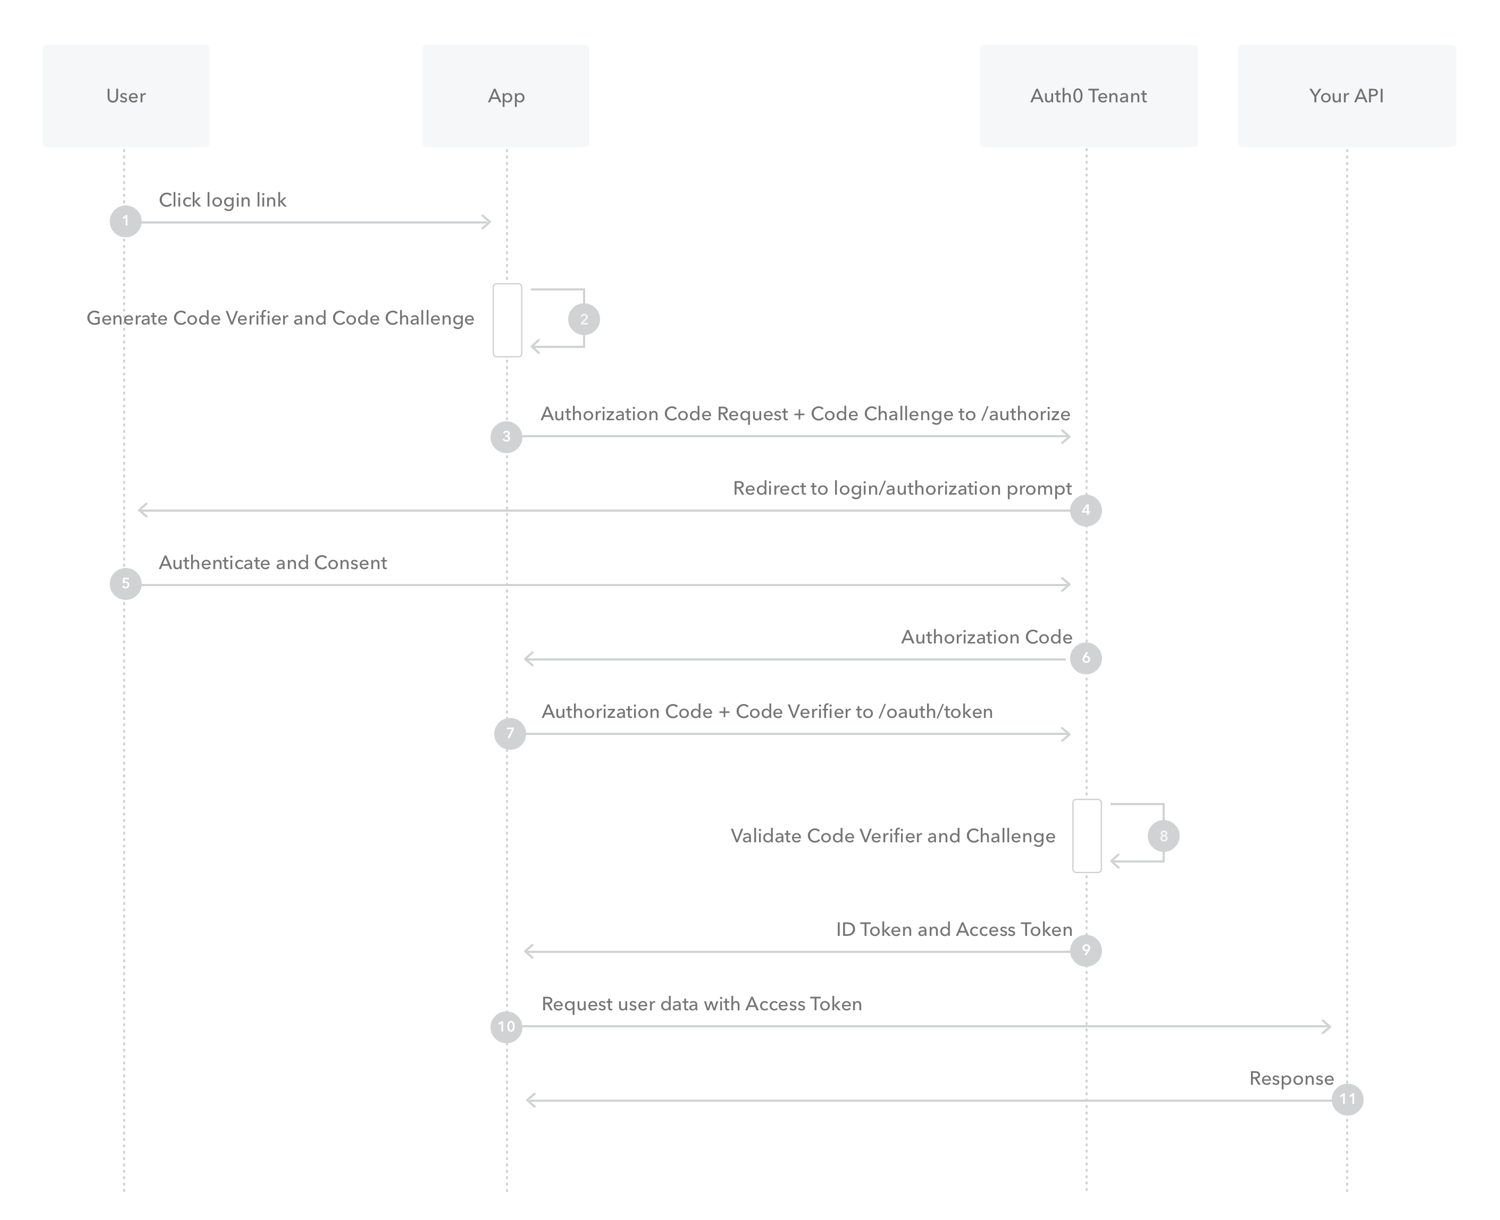
\includegraphics[width=0.85\textwidth]{figures/oauth}
    \caption{Authorization Code Flow with PKCE (source: Auth0 documentation~\cite{auth0PKCE})}
    \label{fig:oauth-flow}
\end{figure}

The IAM module exposes the public keys used for token verification via a JWKS endpoint,
which the API module reads at startup to configure its own authentication filter.

\subsection{The API Module}

\texttt{api} is the core of the application. It is deployed as a WAR under
\texttt{/rest-api} and provides all of the business logic: workspace management,
membership and role administration, epics, tickets, and their associated comments.

Its structure evolved significantly throughout the internship because the project followed
an agile/Scrum approach --- features were added, endpoint contracts revised, and the
authorization model refined sprint by sprint. The module is organized around resource
packages, each containing the endpoint class, DTO definitions, and the specific fetch,
create, update, and delete operations for a given entity (e.g.,
\texttt{EpicEndpoint}, \texttt{TicketEndpoint}, \texttt{MembershipEndpoint}).

Every protected endpoint passes through two Jakarta interceptors before reaching
business logic: an \textbf{authentication filter} that validates the JWT and sets the
caller's identity into a \texttt{ThreadLocal}, and a \textbf{workspace policy
enforcement point} that applies the ABAC rules defined in the core module.

\section{Frontend Architecture: The MVP Pattern}

The frontend is a pure vanilla JavaScript SPA. No framework, no npm dependencies at
runtime --- just ES modules served as static files. The company's constraint on external
JavaScript dependencies was non-negotiable, which meant the usual React or Vue abstractions
were off the table from the start.

In their place, Canny Vision has developed its own lightweight rendering engine built
around the \textbf{Model--View--Presenter (MVP)} pattern~\cite{fowlerMVP}. Getting to
grips with this pattern took a non-trivial amount of time, because it looks familiar on
the surface but enforces a stricter separation than most frontend developers are used to.

\begin{figure}[H]
    \centering
    \includegraphics[width=0.7\textwidth]{figures/mvpArchitecture}
    \caption{MVP architecture of the Canny Vision frontend engine}
    \label{fig:mvp}
\end{figure}

The engine is implemented in \texttt{scripts/mvp.js} and exposes three base classes:

\begin{itemize}
    \item \textbf{Model} extends \texttt{Observable} and is responsible for all API
          communication via a \texttt{callAPI} method. It maintains an internal LRU cache
          with configurable TTL and ETag support, so repeated GET requests do not always
          hit the network.
    \item \textbf{View} extends \texttt{Observable} and owns the DOM. It declares data
          bindings through a \texttt{defineBindings} method and applies them declaratively
          via \texttt{data-bind} attributes, supporting two-way binding for form inputs
          and one-way binding for display elements.
    \item \textbf{Presenter} wires the Model and View together. It registers as an observer
          on both, reacting to state changes from the model and intent events from the view.
\end{itemize}

The \texttt{Broker} class underpins the whole engine: it is a singleton publish/subscribe
bus that decouples the three layers so that neither the model nor the view holds a direct
reference to the other.

\section{Implementation Phases}

\subsection{Phase 0: Discovery and Infrastructure}

The first two weeks were deliberately not spent writing application features. They were
spent reading the existing IAM codebase, running WildFly, understanding how the existing
frontend starter kit was structured, and getting TLS to work end to end. The goal at the
end of this phase was a single, verifiable milestone: a browser sign-in button that
completed the full PKCE flow and landed back on the frontend with a valid JWT in
session storage.

\subsection{Phase 1: End-to-End Authentication}

Once the infrastructure was understood, the first real implementation task was to wire
three things together: the IAM module, a minimal API deployment (a sample Jakarta EE
project used as a scaffold), and the frontend starter kit. The sign-in flow had to work
end to end --- redirect to the IAM's \texttt{/authorize} endpoint, PKCE challenge and
verifier exchange, token returned to the frontend, and the access token attached to
subsequent API requests via the \texttt{Authorization: Bearer} header.

The client-side OAuth 2.0 logic lives in \texttt{scripts/iam.js}. It handles PKCE
code generation using the Web Crypto API, manages the redirect, exchanges the
authorization code for tokens at the \texttt{/oauth/token} endpoint, and stores the
result in session storage. It also handles token refresh on a background interval and
exposes a \texttt{checkSession} helper used by every page on load.

\subsection{Phase 2: Iterative API Development}

With authentication working, the focus shifted to the API module. Features were built
incrementally across Scrum sprints: workspace CRUD, membership management with role
assignment, the epic hierarchy, ticket management with assignment and status tracking,
and finally the comment system. At each step the ABAC policy was extended to cover the
new resources.

The endpoint contract changed multiple times as the team's understanding of the domain
deepened. The DTO structure, the role permissions matrix, the handling of workspace-scoped
identity (the membership token issued by the IAM alongside the access token) --- all of
these were refined through discussion and iteration rather than designed upfront in full.

\section{Chapter Conclusion}

Setting up the environment consumed more calendar time than anticipated, primarily because
WildFly and TLS-related issues required careful investigation rather than quick fixes.
That investment paid off: once the infrastructure was stable, the iterative feature
development proceeded smoothly, with each sprint delivering a functional increment. The
following chapter presents the results of that work through test scenarios, functional
walkthroughs, and a documented investigation into the most significant technical problem
encountered during integration.

% ============================================================
% RAW NOTES — kept for reference, not included in output
% ============================================================
% the first 2 week at canny vision were solely to understand the existing infrastructure
% I switched my os version from windows to linux to use wildfly effectively and set up the server
% talk about the stenghts of wildfly and how it's not your everyday server and how hard is it to set it up
% you can talk about how I spent 3 days trying to solve a problem where the server didn't allow cors request from the frontend to the api
% and how finally the problem was that the certficate used was created by sudo (sudo user) and when I set it up I used normal user
% ->so there was a mix in the certfifs :
% You were using mkcert to secure your local environment (iam.localhost). Even though you successfully imported the certificates into the Oracle JDK cacerts file using keytool, your Java code continued to throw SSLHandshakeException.
%
% (please read /middleware/core/configs to understand more)
% even though I didn't develop myslef the IAM module, understanding it was not an easy task
%
% the official documentation link to be included : https://auth0.com/docs/get-started/authentication-and-authorization-flow/authorization-code-flow-with-pkce
% I added on the figures folder an image figures/oauth that explain the flow of the authentication and authorization process in the system
%
% so my first task was to have a connecting iam module , api module (just old examlpe project) and frontend (just a starter kit with an mvp page example)
% and have a working sign -in flow
% I spent a hell of time understanding how the mvp patter work
% (I will provide in figures an image showing the architecure of mvp)
% (read from frontend/scripts/mvp.js to understand more)
% and read /frontend/scripts/iam.js to see how the iam connects to the frontned
%
% after getting the grasp of how everything works
% I started to implement the api module which is the core of the system
% and which its architectuee has changed many times during the internship since we worked in agile/scrum
% and kept on adding features and improving the design as we went along
%
% please talk about the folder strcuture of the middleware :
% how I used maven pom.xml to manage dependencies and build the project
% with three main modules : core, api and iam
% (read the folder middleware to understand more about the structure and the content of each module)
% talk about how core is the jar that contains all the common code and utilities that are shared between the api and iam modules
% and how the api module contains the business logic and the REST endpoints
% and how the iam module contains the authentication and authorization logic
%
% dear claude please take note that I am just throwing ideas ; and decide yourself the best order of the content
